%%%%%%%%%%%%%%%%%%%%%%%%%%%%%%%%%%%%%%%%%%%%%%%%%%%%%%%%%%%%%%%%%%%%%%%%%%%%%%%%%%%%%%%%%%%%%%%%%%%%%%%%%%%%%%%%%%%%%%%%%%%%%%%%%
\chapter{On the Server Side}
\label{cha:on_the_server_side}

%%%%%%%%%%%%%%%%%%%%%%%%%%%%%%%%%%%%%%%%%%%%%%%%%%%%%
\section{Architecture}

In order to retrieve information about nearby stops, the client must request a remote source of information by calling a server. The server that has been implemented in our case acts as a middleware between the public transport providers (Västtrafik and SL) and the client. By doing so, requests to the different providers are transparent to the client.\\

The server processes a request for nearby bus stops as follows:

\begin{enumerate}
\item{it receives a request with coordinates (Latitude and Longitude)}
\item{it finds the 10 nearest bus locations from the given coordinates in its SQLite database}
\item{it fetches the forecast for each of these stops in an independent lightweight process}
\item{once each forecast is obtained, it parses the result into JSON format}
\item{finally, it sends a reply to the client containing the JSON data}
\end{enumerate}

In order to handle high quantities of lightweight processes, the best solution was to use Erlang. Erlang is a functional programming language especially designed to handle high concurrency and distributed systems.  A large part of the application is therefore implemented in Erlang in order to take advantage of this.\\

Figure \ref{fig:message_passing} shows in details the request processing on an UML sequential diagram, the grey area being our server.

\begin{figure}[ht]
\center
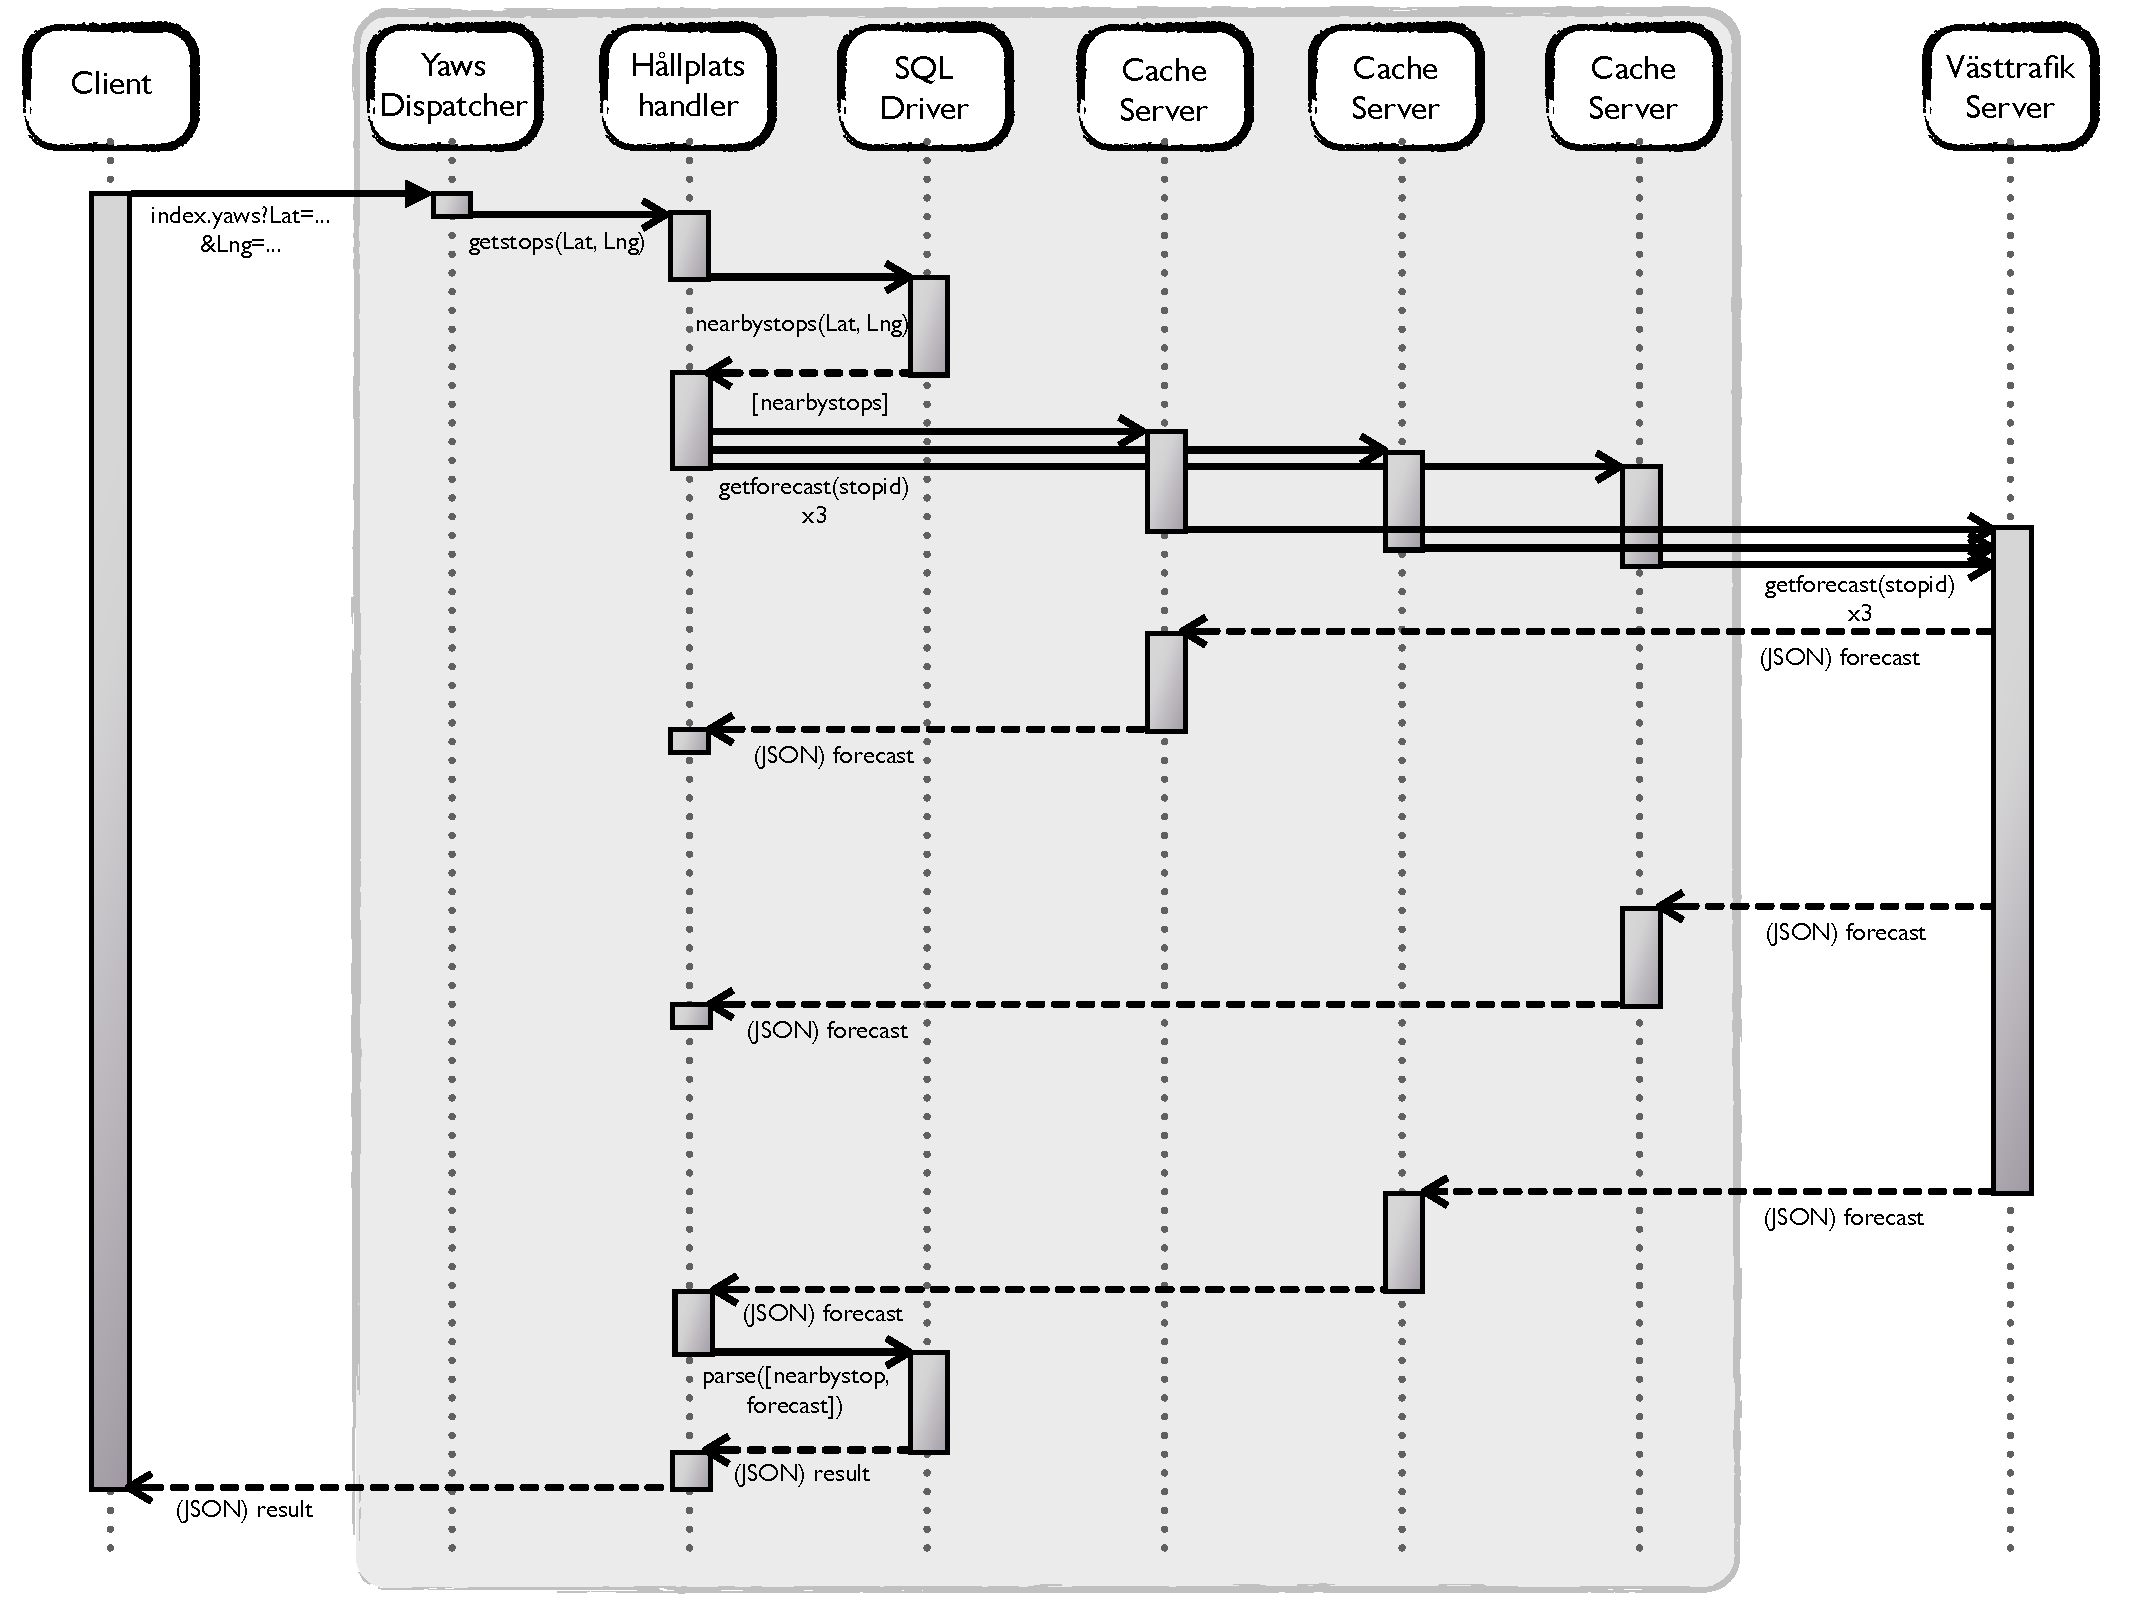
\includegraphics[scale=0.4]{pics/message_passing}
\caption{Simplified UML Sequential Diagram of a request}
\label{fig:message_passing}
\end{figure}

\clearpage

The application is hosted on a Debian machine (Ubuntu) with a Yaws webserver. Yaws is the Erlang alternative to Apache, and as such offers high availability and high scalability.\\

But to make it easy to maintain and update, the more complex tasks are implemented in Ruby. Ruby is a modern dynamic scripted language, and has been designed to make the developers happy. As such, it is a powerful tool to implement complex algorithms painlessly.\\

Figure \ref{fig:server_architecture} shows the details of the server's architecture.

\begin{figure}[ht]
\center
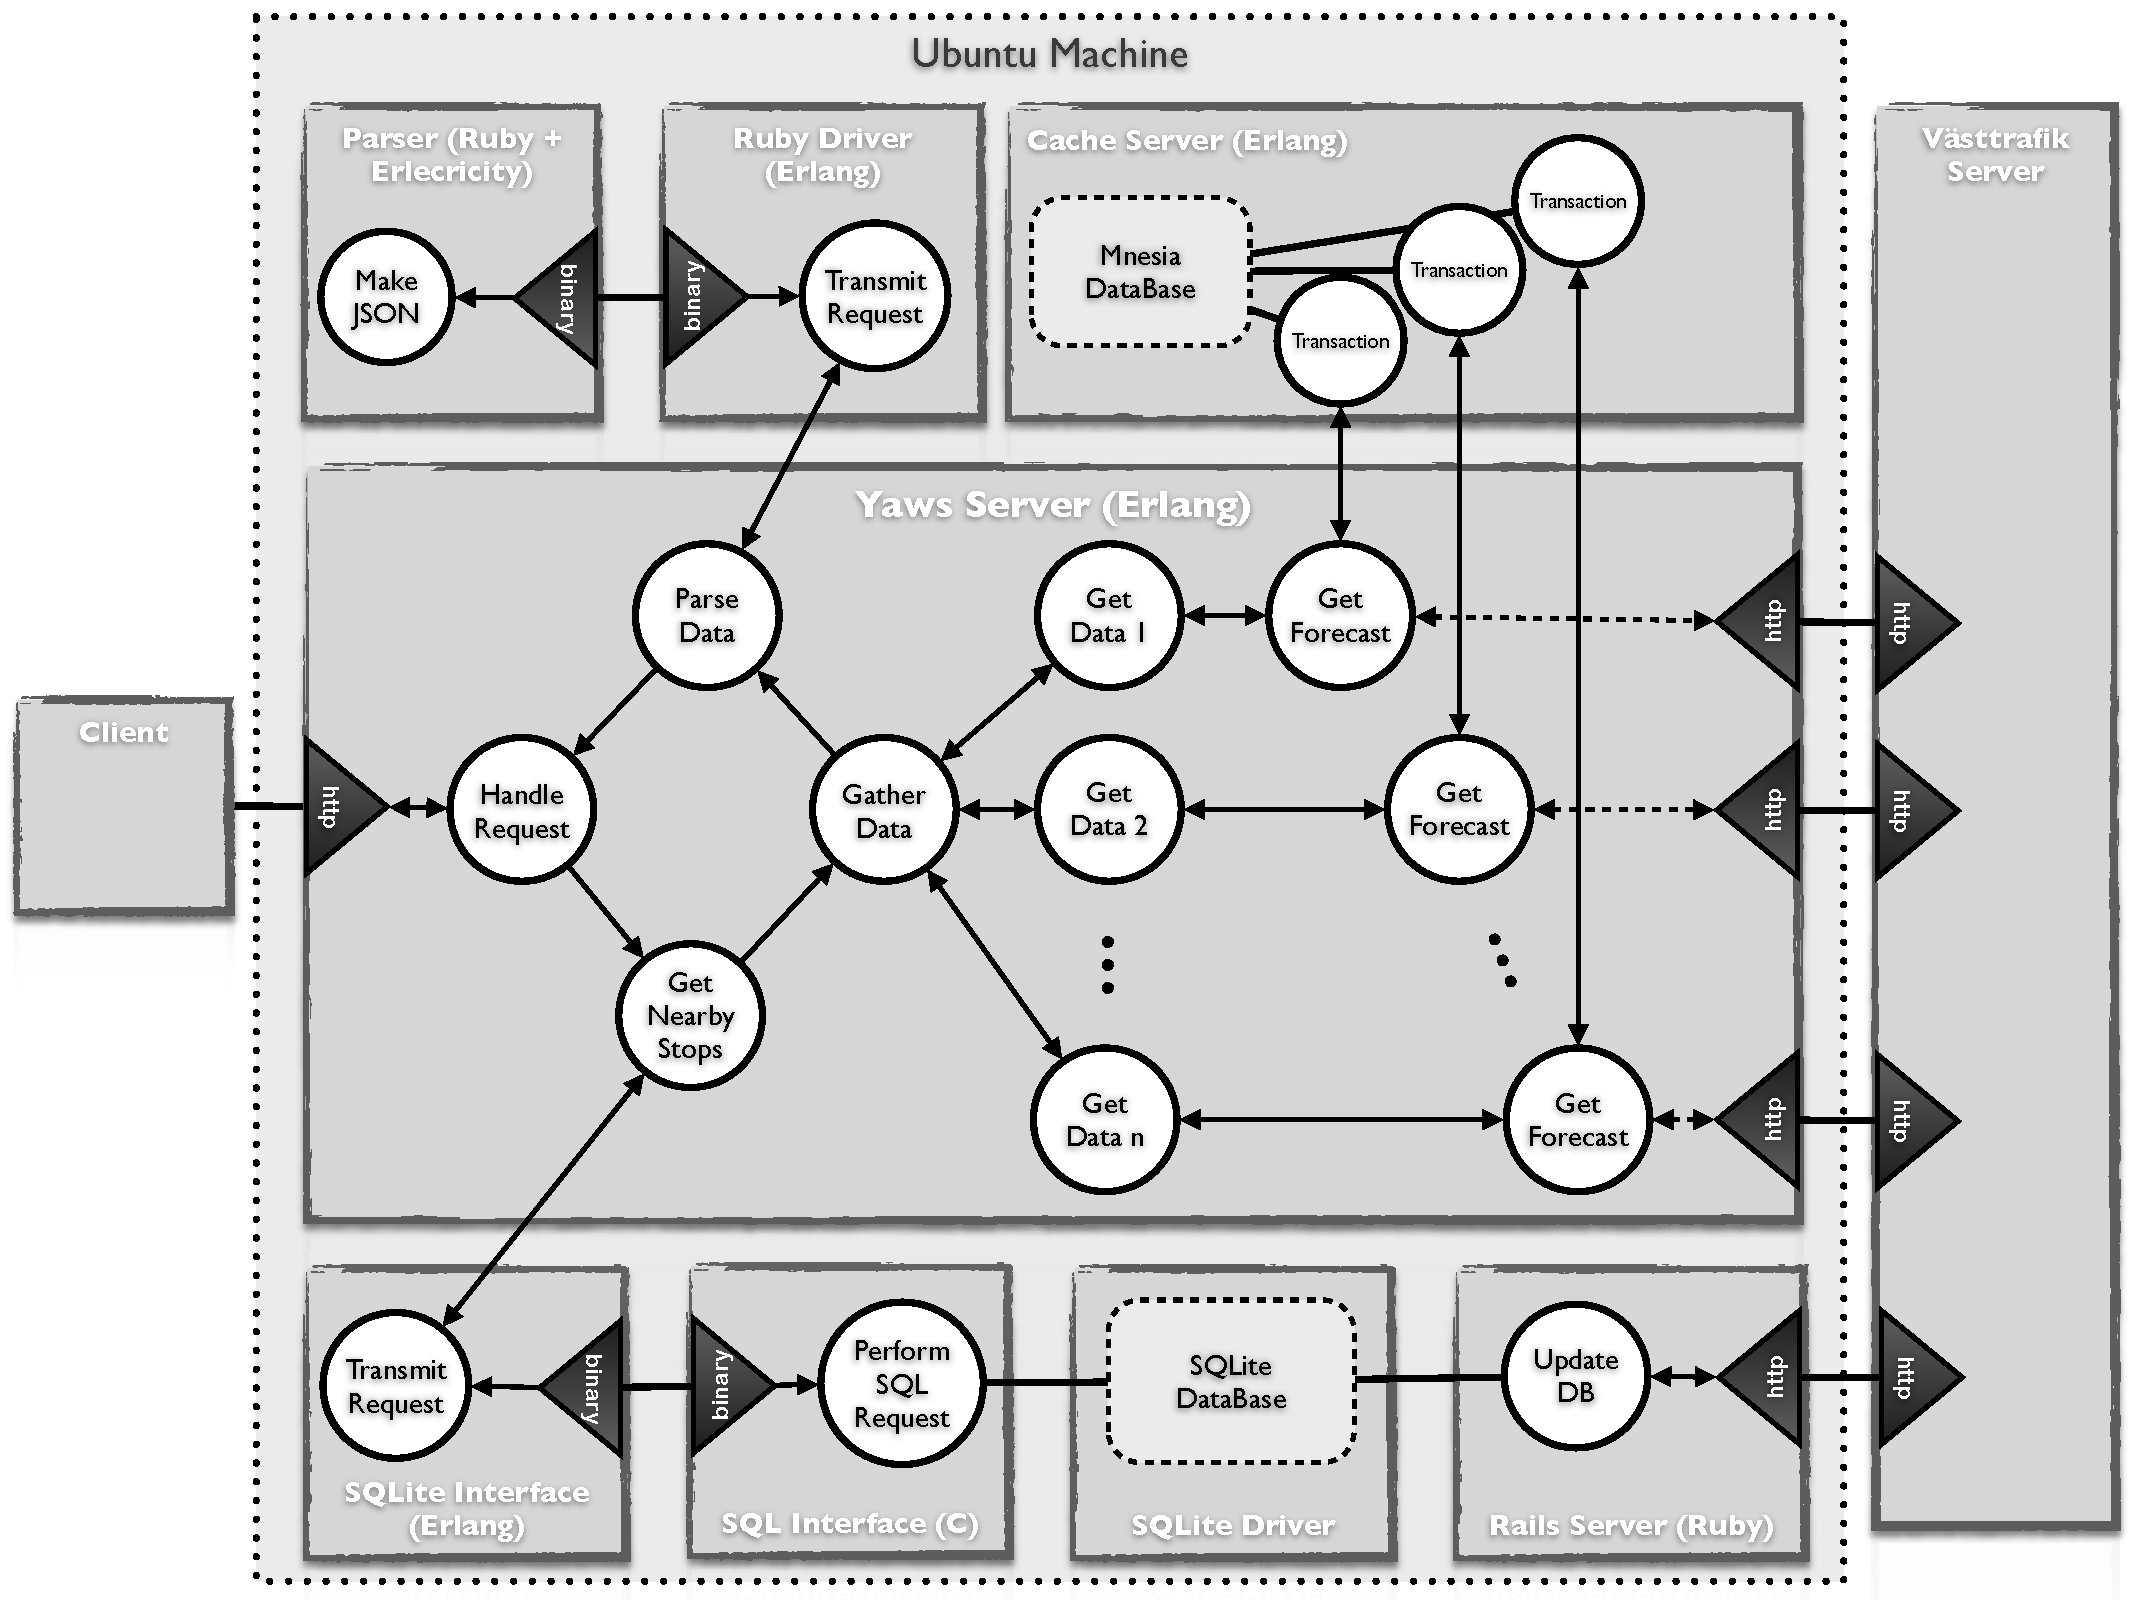
\includegraphics[scale=0.4]{pics/server_side}
\caption{Scheme of the Server Architecture}
\label{fig:server_architecture}
\end{figure}

\clearpage

%%%%%%%%%%%%%%%%%%%%%%%%%%%%%%%%%%%%%%%%%%%%%%%%%%%%%
\section{Implementation}


\subsection{Erlang}

Erlang is used to dispatch the lightweight processes, to perform the distant requests to Västtrafik and Storstockholms Locaktrafik, and also to take care of data caching by the mean of a Mnesia database.

\subsection{Ruby}

Ruby is used to implement the SQL request to the database and to parse data. It is also used to maintain the database. The SQL database contains information on all the bus stops for each provider. Each entry in the database has the following attributes:

\begin{tabular}{ l l l l }
$\bullet$ & stop\_name 	& : & the name of the stop\\
$\bullet$ & lat 			& : & the Latitude of the stop\\
$\bullet$ & lng 			& : & the Longitude of the stop\\
$\bullet$ & provider\_name & : & the name of the stop's provider (Västtrafik or SL)\\
$\bullet$ & stop\_id 		& : & the id of the stop as defined by its provider\\
\end{tabular}\\

This database is populated by a background process that fetch data from the providers on monthly basis (it is not that often that new stops are build or that old one are destroyed).\\

The "lat" and "lng" attributes are the key entries allowing geographic search in the database, but finding nearby points from a database can be a tricky problem. In our case, we perform queries iteratively as shown in Figure \ref{fig:ruby_queries} until a satisfying number of stops are returned.

\begin{figure}[ht]
\subfigure[Step 1]{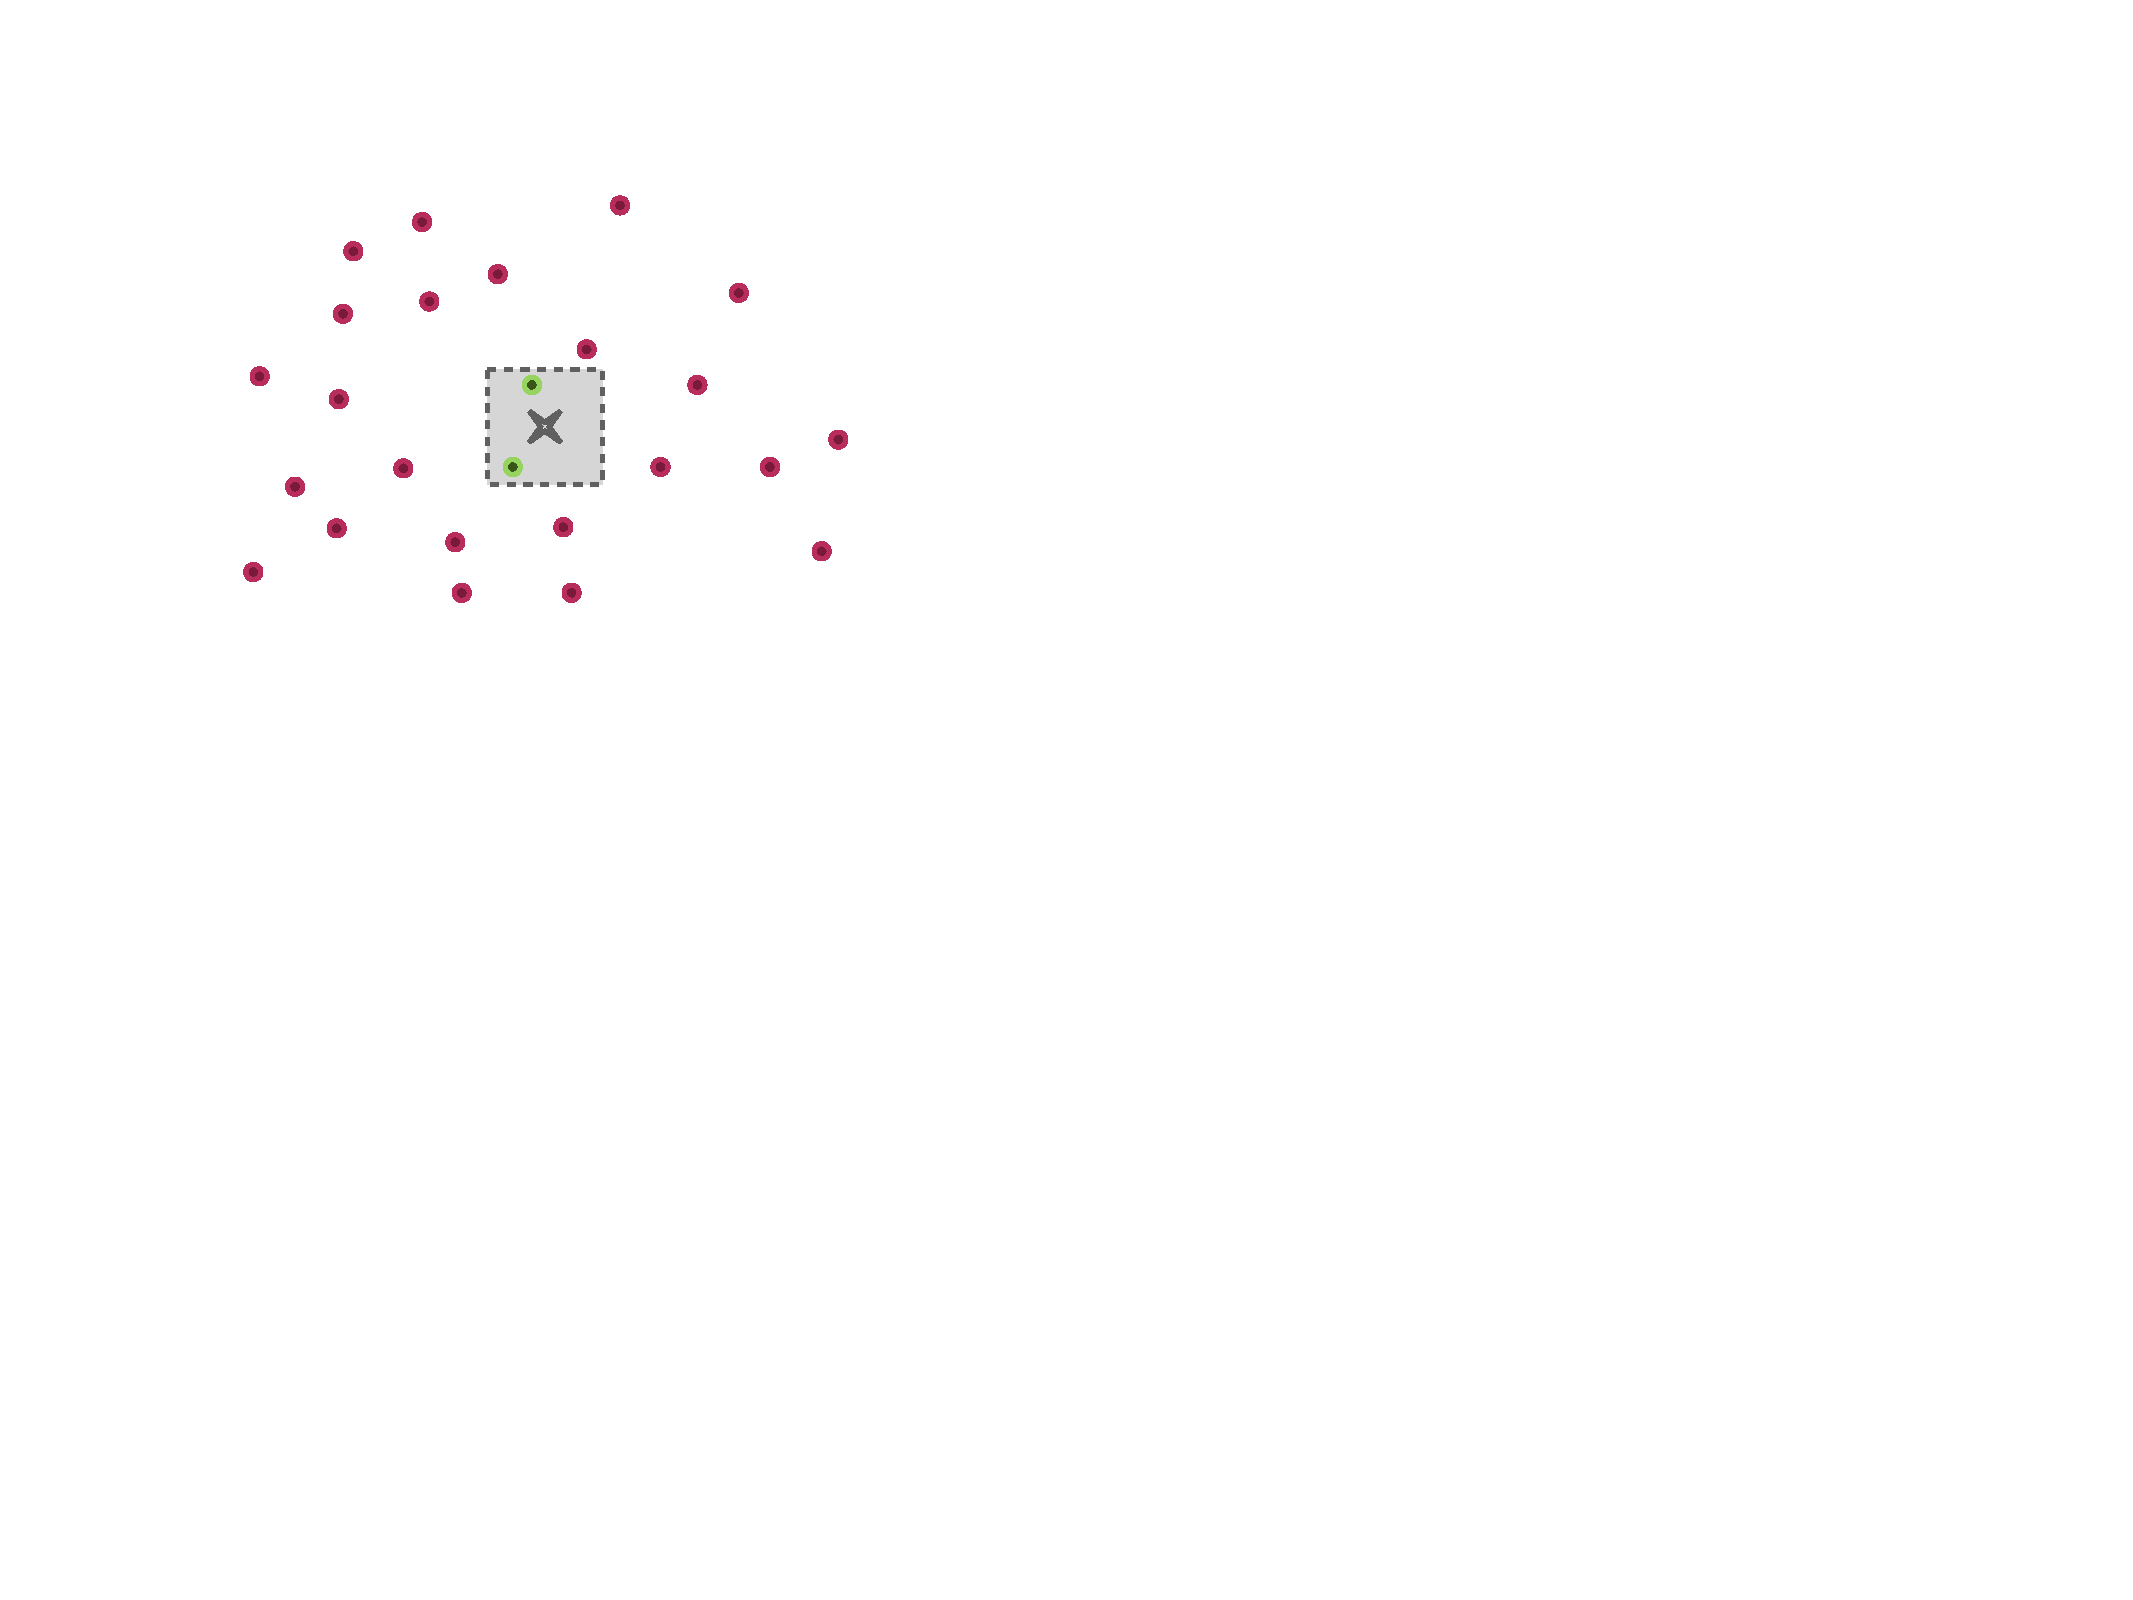
\includegraphics[scale=0.5]{pics/ruby_query_1}}
\hspace{0.1cm}
\subfigure[Step 2]{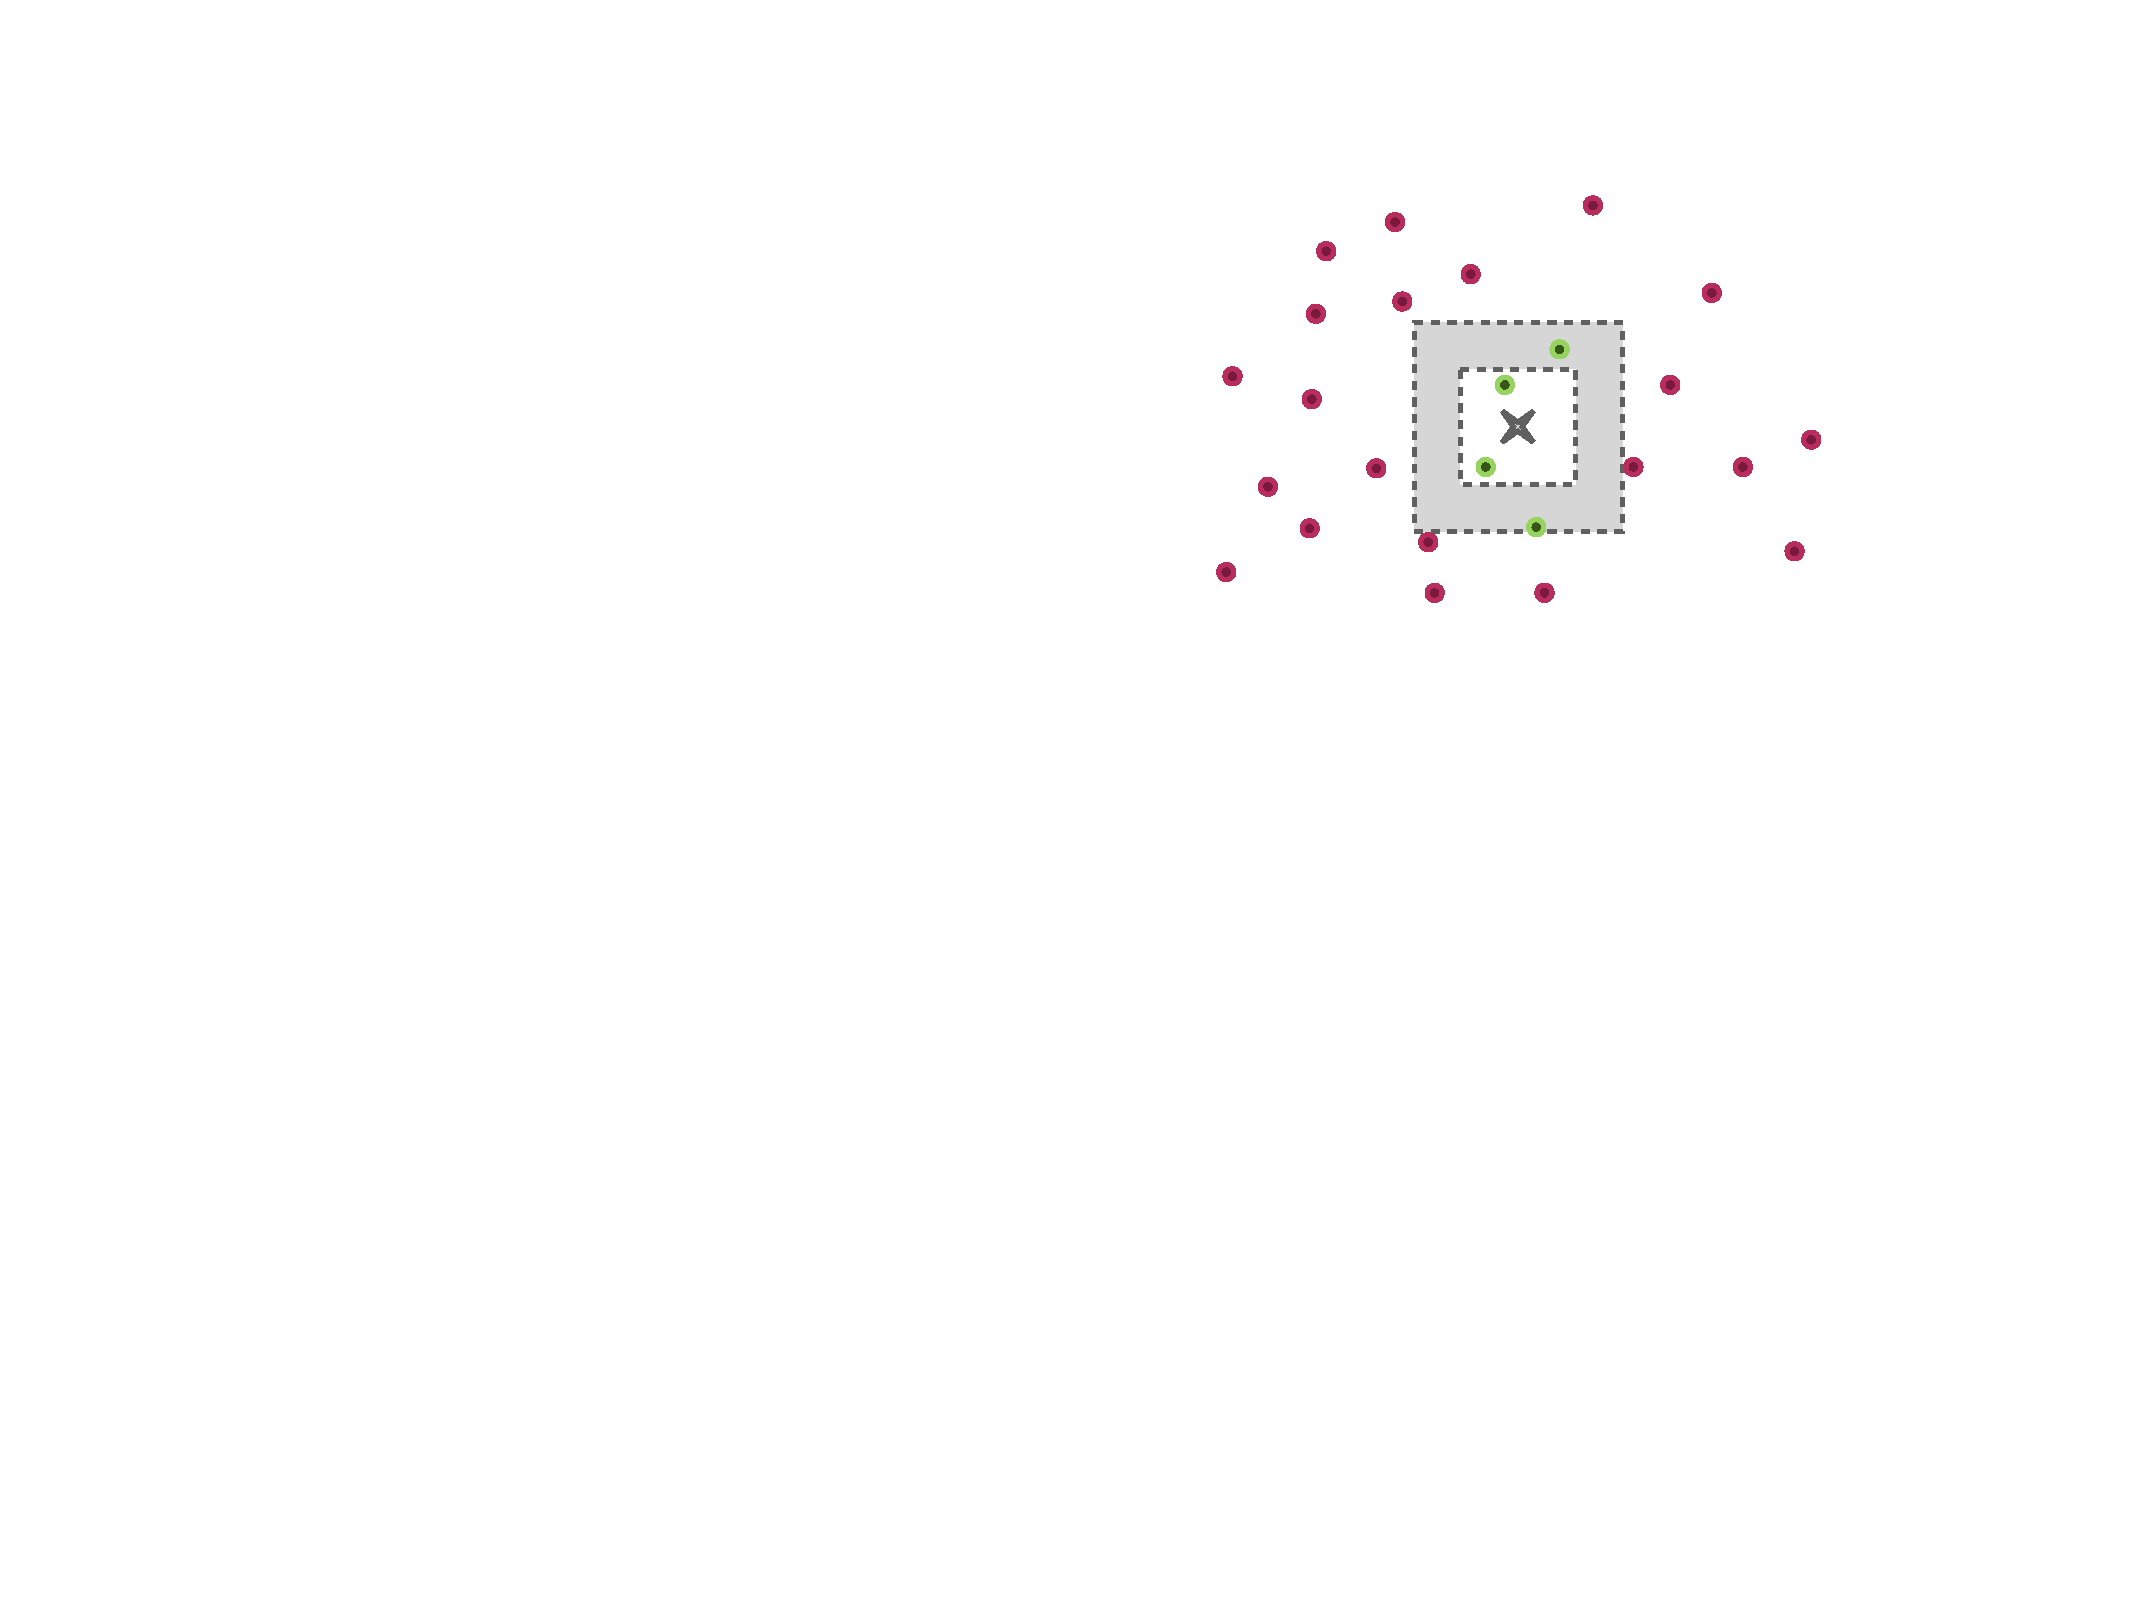
\includegraphics[scale=0.5]{pics/ruby_query_2}}
\hspace{0.1cm}
\subfigure[Step 3]{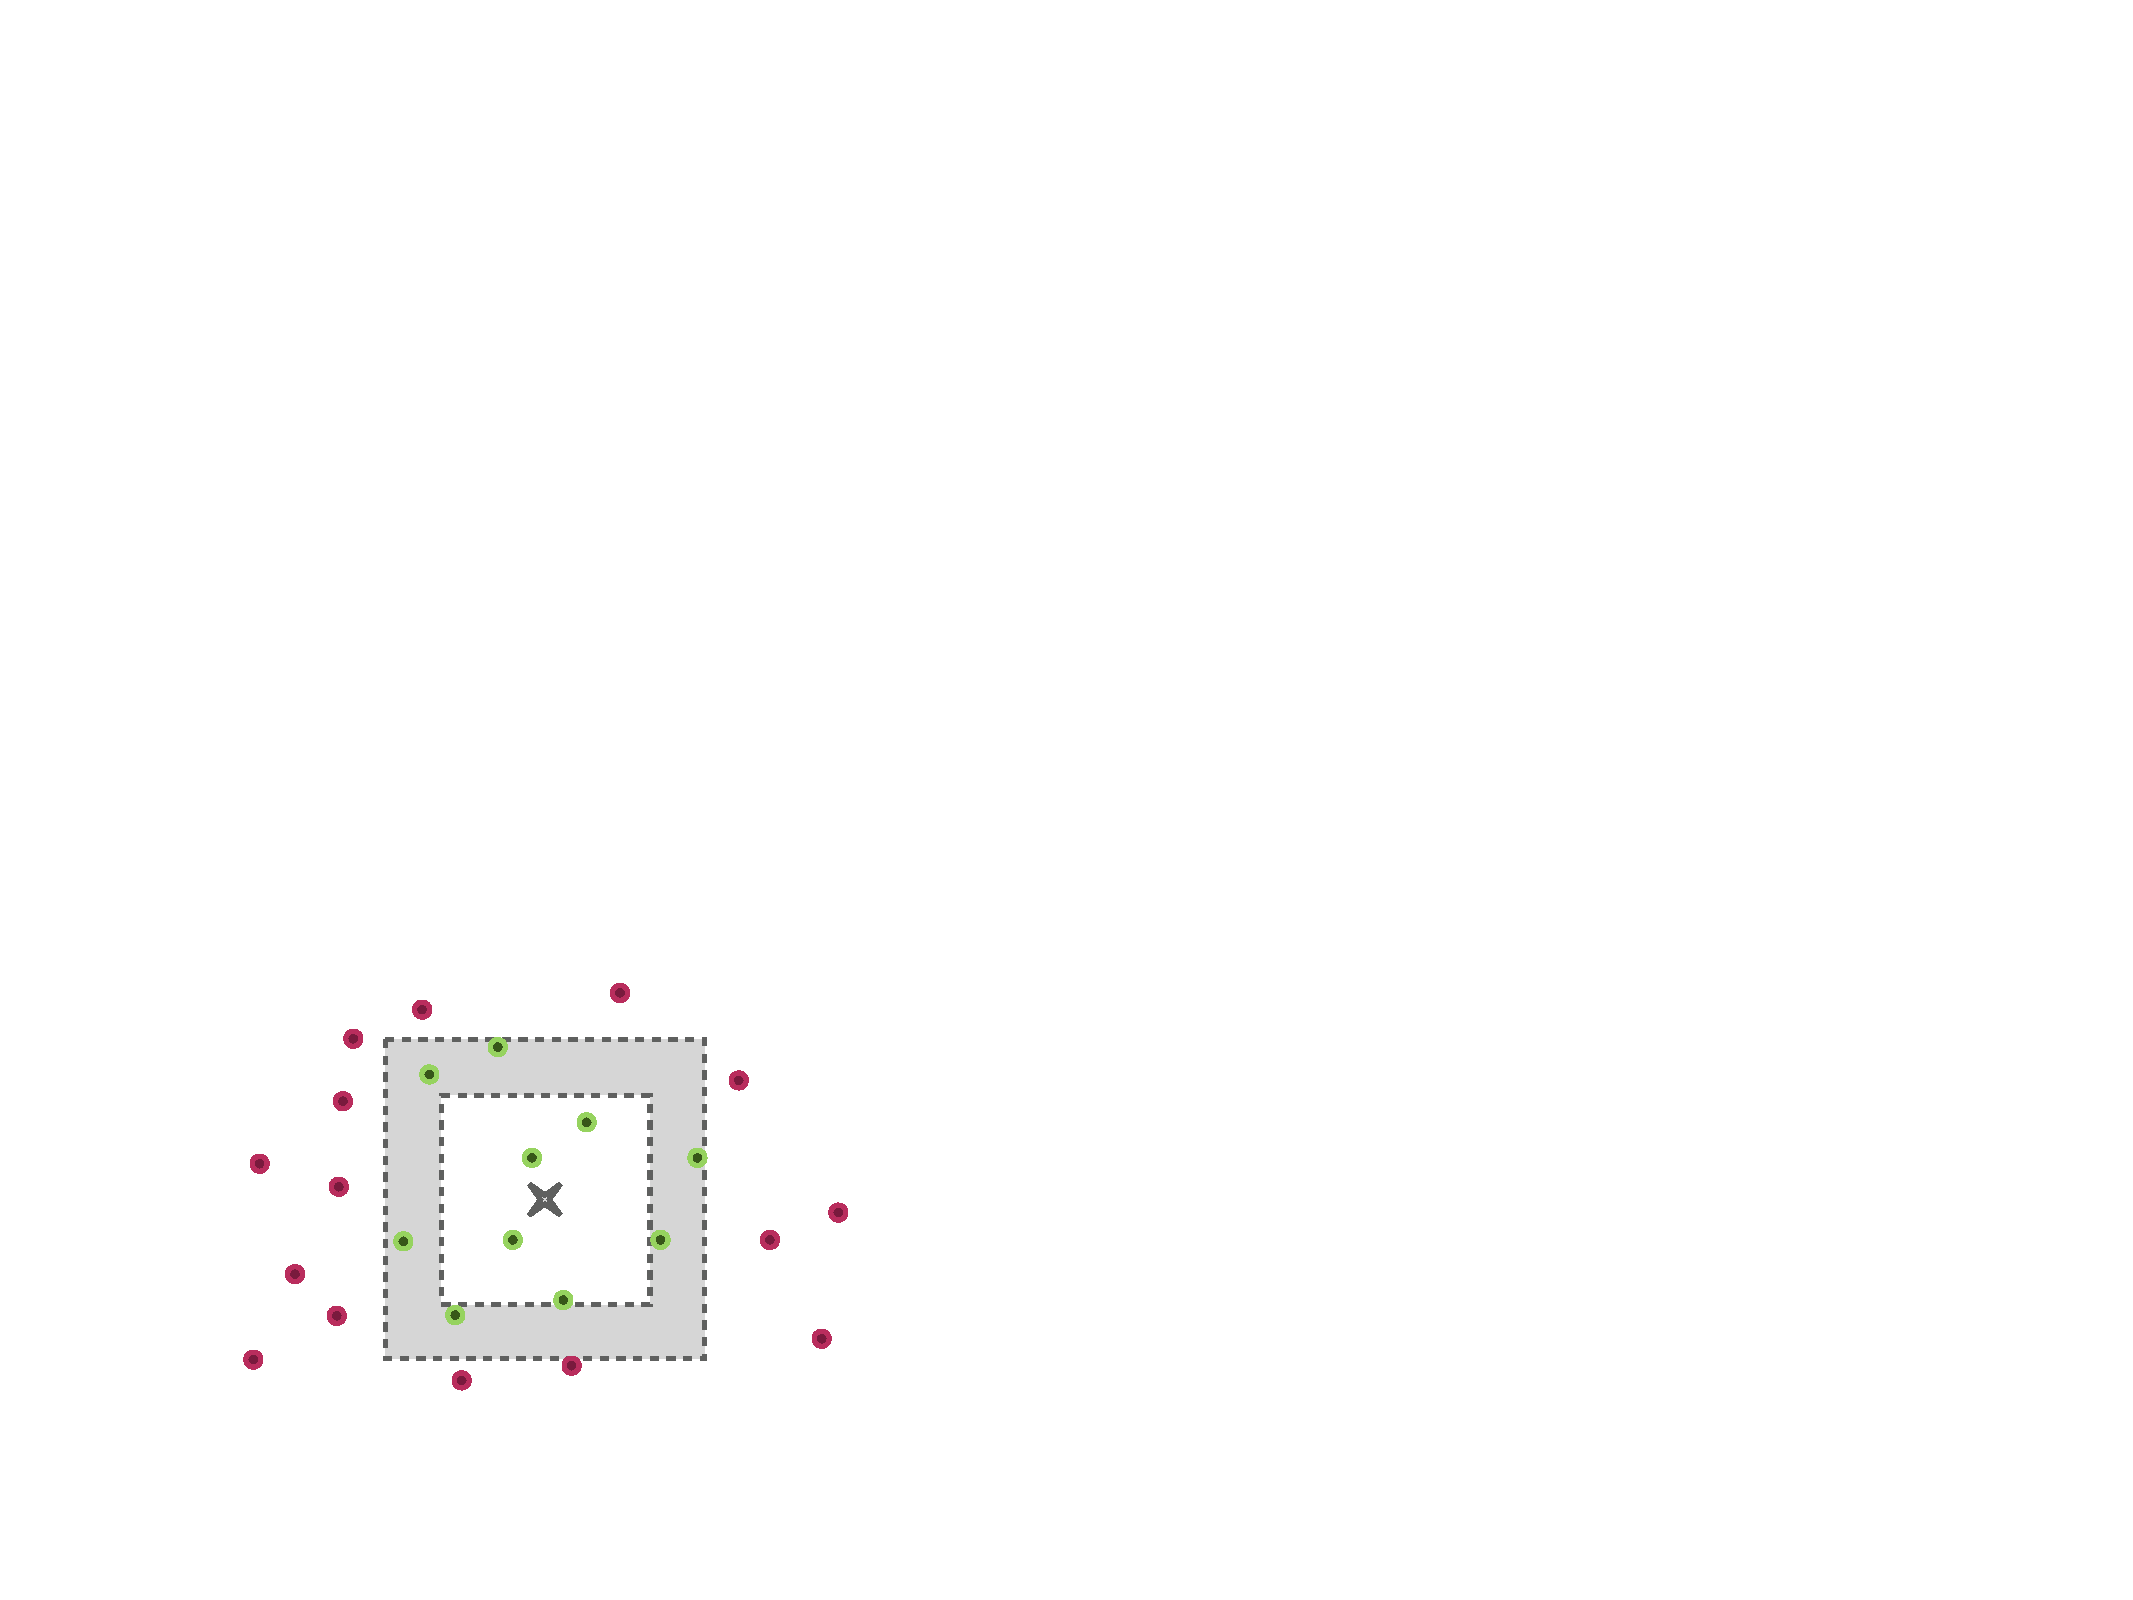
\includegraphics[scale=0.5]{pics/ruby_query_3}}
\caption{Scheme of the SQL queries on the Ruby side}
\label{fig:ruby_queries}
\end{figure}

Once we get a list of stops within an arbitrary large area, we need to sort those stops by distance in order to keep only the 10 closer ones. The distance $d$ between the user's location and a stop is computed according to a simplified version of the great-circle distance formula given in Equations \ref{equ:great_circle_formula_1} and \ref{equ:great_circle_formula_2}, where $\phi_s$ and $\lambda_s$ are the Latitude and Longitude of the standpoint, $\phi_f$ and $\lambda_f$ the ones of the forepoint, with $\Delta \hat{\sigma}$ defining the central angle of those two points and $r$ being the average radius of Earth ($\approx6371$km).

\begin{equation}
\label{equ:great_circle_formula_1}
\Delta \hat{\sigma} = \textrm{arccos}\left(\textrm{cos}\phi_s \textrm{ cos}\lambda_s \textrm{ cos}\phi_f \textrm{ cos}\lambda_f + \textrm{cos}\phi_s \textrm{ sin}\lambda_s \textrm{ cos}\phi_f \textrm{ sin}\lambda_f + \textrm{ sin}\phi_s \textrm{ sin}\phi_f\right)
\end{equation}

\begin{equation}
\label{equ:great_circle_formula_2}
d = r \times \Delta \hat{\sigma}
\end{equation}

%%%%%%%%%%%%%%%%%%%%%%%%%%%%%%%%%%%%%%%%%%%%%%%%%%%%%
\section{Results}

Everything works fine.

(give numbers)